\documentclass[10pt]{beamer}

\usetheme[progressbar=frametitle]{metropolis}
\usepackage{appendixnumberbeamer}
\usepackage[utf8]{inputenc} %Required for encoding text
\usepackage[french]{babel}
\usepackage{booktabs}
\usepackage[scale=2]{ccicons}

\usepackage{pgfplots}
\usepgfplotslibrary{dateplot}
\usepackage{xspace}

\usepackage{xcolor}
\usepackage{listings}
\usepackage{tcolorbox}
\tcbuselibrary{listings,skins}
%\lstset{basicstyle=\ttfamily\color{white},
%  showstringspaces=false,
%  xleftmargin = 0.5cm,
%  commentstyle=\color{red},
%  keywordstyle=\color{blue},
%  rulecolor=\color{white},
%  frameshape={RYR}{Y}{Y}{RYR},
%  backgroundcolor=\color{black},
%}
\lstdefinestyle{mystyle}{
     basicstyle=\ttfamily\color{white},
     language=bash,
     tabsize=1,
     keywordstyle=\color{blue}\bf,
     showstringspaces=false,
     morekeywords={mount, umount, ls, 
	 		cat, adduser, chown, chgrp, init, fuser}
 }
\newtcblisting{mylisting}{
      enhanced,                             %%% needed for shadow
      arc=2mm,
      top=0mm,
      bottom=0mm,
      left=0mm,
      right=0mm,
      boxrule=0pt,
      colback=black,
      %shadow={5mm}{-3mm}{0mm}{fill=black!50!white,opacity=0.5},             %%% here for shadow  and adjust as you like
      listing only,
      listing options={style=mystyle},
      hbox
}

\newcommand{\linux}{\textbf{\textsc{Linux}}\xspace}
\newcommand{\param}[1]{\textcolor{blue}{#1}}

\addtobeamertemplate{section page}{}{
  \centering
  \begin{minipage}{22em}
  \tableofcontents[sectionstyle=hide/hide,hideothersubsections]
  \end{minipage}\par
}
\title{Introduction à Linux}
\subtitle{Cours d'Outils de Programmation}
% \date{\today}
\date{}
\author{Bousbaa Imad Eddine}
\institute{Université des Sciences et de la Technologie de Houari Boumediène}
% \titlegraphic{\hfill\includegraphics[height=1.5cm]{logo.pdf}}

\begin{document}

\maketitle

\begin{frame}{Plan}
  \setbeamertemplate{section in toc}[sections numbered]
  \tableofcontents[hideallsubsections]
\end{frame}

\section{}

\begin{frame}[fragile]{Objectifs}

Avoir une idée du libre et comment donner une licence à sont travail.

Permettre à un utilisateur Linux de se familiariser à l'utilisation et la personnalisation d'un
système Linux.\\

\end{frame}

\section{Le libre}
\subsection{Le mouvement GNU}
\begin{frame}[fragile]{Qu'est ce que le mouvement GNU ?}

  En 1984, Richard Matthew Stallman, chercheur en informatique du MIT quitte son
poste et se consacre à l’écriture d’un système d’exploitation Libre du nom de GNU .
Il annonce l’année suivante la création de la FSF afin de supporter ce projet.
C'est durant ces années qu'il écrit ce qui deviendra les préceptes du Logiciel Libre.
La concrétisation en est la publication en 1989 de la première version de la licence
GPL qui sera alors le fondement éthique, juridique et politique du mouvement du
Libre. 

Plus d’information sur le mouvement GNU sur le site http://www.gnu.org/ .
\end{frame}

\begin{frame}[fragile]{Qu'est-ce qu'un logiciel libre ?}
L'expression « Logiciel Libre » fait référence à la liberté et non pas au prix. Pour
comprendre le concept, vous devez penser à la « liberté d'expression », pas à «
l'entrée libre ».

L'expression  «  Logiciel  Libre   »  fait  référence   à  la  liberté  pour   les utilisateurs
d'exécuter, de copier, de distribuer, d'étudier, de modifier et d'améliorer le logiciel.
\end{frame}
\begin{frame}

Plus précisément, elle fait référence à quatre types de liberté pour l'utilisateur du
logiciel :

\begin{definition}
	\begin{enumerate}
		\item La liberté d'exécuter le programme, pour tous les usages.
		\item La liberté d'étudier le fonctionnement du programme, et de l'adapter à vos besoins. Pour ceci l'accès au code source est une condition requis.
		\item La liberté de redistribuer des copies, donc d'aider votre voisin.
		\item La liberté d'améliorer le programme et de publier vos améliorations, pour en faire profiter toute la communauté. Pour se faire, l'accès au code source est une condition requise.
	\end{enumerate}
\end{definition}
\end{frame}

\begin{frame}{Classification des logiciels}
	\begin{tabular}{c|cccc}
			& Utiliser & Copier & Modifier & redistribuer \\
	propriétaire & \textcolor{green}{oui}, \textcolor{red}{si tu payes} & \textcolor{red}{non} & jamais & jamais \\
	Shareware & \textcolor{green}{oui} \textcolor{red}{(période d'essai)} & \textcolor{red}{non} & \textcolor{red}{non} & \textcolor{red}{non} \\
	Freeware & \textcolor{green}{oui} & \textcolor{green}{oui} & \textcolor{red}{non} & \textcolor{red}{non}\\
	libre & \textcolor{green}{oui} & \textcolor{green}{oui} & \textcolor{green}{oui} & \textcolor{green}{oui}
	\end{tabular}
\end{frame}


\begin{frame}{Pas que le logiciel}
La philosophie du Libre touche aujourd’hui d’autres domaines :
	\begin{itemize}
		\item l’art (musique, livres, images) avec les licences Creative Commons,
		\item le partage du savoir avec l’encylopédie collaborative Wikipedia,
		\item les publications scientifiques,
		\item différents moyens techniques et recettes,
		\item etc.
	\end{itemize}
\end{frame}
\subsection{Creative Commons}
\begin{frame}{Creative Commons : Les attributs}
	\begin{itemize}
		\item \textbf{Paternité [BY] (Attribution) :} l'œuvre peut être librement utilisée, à la condition de l'attribuer à l'auteur en citant son nom. 
		\item \textbf{Pas d'utilisation commerciale [NC] ( Noncommercial ) :} le titulaire de droits peut autoriser tous les types d’utilisation ou au contraire restreindre aux utilisations non commerciales (les utilisations commerciales restant soumises à son autorisation). 
		\item \textbf{Pas de modification [ND] ( NoDerivs ) :} le titulaire de droits peut continuer à réserver la faculté de réaliser des œuvres de type dérivées ou au contraire autoriser à l'avance les modifications, traductions. 
		\item \textbf{Partage des conditions initiales à l'identique [SA] ( ShareAlike ) :} le titulaire des droits peut autoriser à l'avance les modifications ; peut se superposer l'obligation (SA) pour les œuvres dites dérivées d'être proposées au public avec les mêmes libertés (sous les mêmes options Creative Commons) que l'œuvre originale. 
	\end{itemize}
\end{frame}
\begin{frame}{résumé}
	\begin{center}	
		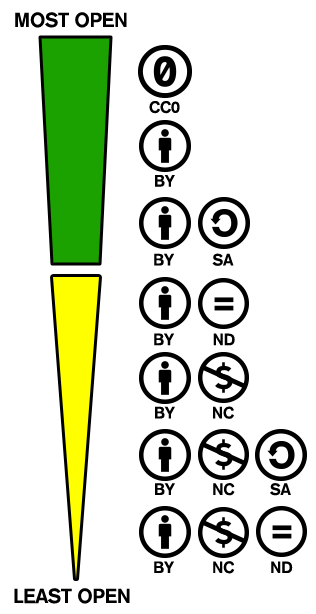
\includegraphics[height=6cm]{img/cc.png}
	\end{center}
\end{frame}
\section{Linux}
\subsection{Historique et définitions de base}
\begin{frame}{\linux, juste le noyau !}

«Au sens strict, \linux est le nom du noyau de système d'exploitation libre, multitâche multiplate-forme et multi-utilisateur de type UNIX créé par Linus Torvalds, souvent désigné comme le noyau Linux. »

Le projet GNU arrive en 1991 avec de très nombreux outils libres, mais il lui manque un élément central : le noyau. Cet élément est essentiel car il gère la mémoire, le microprocesseur, les périphériques comme le clavier, la souris, les disques durs\ldots

C'est à cette époque qu'un étudiant finlandais, Linus Torvalds, commence à développer un noyau et demande aux personnes intéressées d'y contribuer. La licence GPL a été publiée à la même époque et Linus Torvalds s'est laissé persuader de placer son noyau sous cette dernière. 
Le système d'exploitation actuellement connu est donc un assemblage des outils GNU fonctionnant sur un noyau Linux, on parle donc de GNU/Linux avec le slash, « / » pour « GNU sur Linux ».

\end{frame}

\begin{frame}
\begin{alertblock}{En résumé}
GNU/Linux est un système d'exploitation complètement Libre et performant. Il est
hautement configurable. Il ne dépend pas d'une multinationale. Il est supporté par
une grande communauté d'utilisateurs souvent prêts à vous aider. Quelque soit
votre   domaine   de   compétence,   vous   pouvez   participer   à   l'amélioration   de
GNU/Linux pour que ce dernier évolue dans votre intérêt. Ce n'est pas un simple
logiciel gratuit, mais un Logiciel Libre. Ce qui garantit qu'il restera accessible et
gratuit pour tous, sans discrimination.
\end{alertblock}
\end{frame}

\begin{frame}{Qu'est ce qu'une distribution ?}
En réalité, si on vous livrait le noyau Linux seul, accompagné des outils GNU de base, vous seriez bien avancé : pas d'interface graphique, juste quelques commandes, bref, votre système d'exploitation serait inexploitable, un comble,non ?

C'est pour cela qu'existe des distributions Linux qui contiennent le noyau Linux, les outils GNU, plus un ensemble de logiciels qu'elles ont choisi de supporter. Ceux-ci sont testés et compilés pour vous. La plupart d'entre elles contiennent un système d'installation de logiciel simplifié qui leur est – malheureusement – propre. Vous avez déjà dû voir qu'il existe de très nombreuses distributions
: Mandriva, Red Hat Fedora, Debian, Gentoo, OpenSuse, Ubuntu ... 
\end{frame}

\begin{frame}{Qu'est ce qu'une distribution ?}
Pourquoi autant de distributions ? 

En fait, chaque distribution a sa cible: certaines sont orientées sur la facilité d'utilisation,d'autres sont pour les véritables «geeks», certaines sont spécialisées pour l'utilisation dans le domaine scolaire ou musical, d'autres encore se veulent très légères et fonctionner sur des
PC antédiluviens\ldots.
\end{frame}

\begin{frame}{À quoi sert vraiment un système d'exploitation?}
Il exploite ! Oui, mais « qui » allez-vous me dire ? En fait, il s'agit plutôt de «quoi» : l'OS exploite votre matériel.

\pause
Essayons d'imaginer le contraire: si le système d'exploitation n'existait pas, tous
les logiciels devraient être conçus pour tous les matériels existants.

C'est à dire que chaque programmeur devrait prendre en compte l'ensemble du matériel (carte graphique,type de mémoire RAM, disque dur, processeur. . .) ainsi que tous les périphériques
( clavier, souris, écran, imprimante. . .) existant ou ayant existé.
\end{frame}

\begin{frame}{À quoi sert vraiment un système d'exploitation?}
Essayons d'imaginer le contraire : si le système d'exploitation n'existait pas, tous
les logiciels devraient être conçus pour tous les matériels existants. C'est à dire que chaque programmeur devrait prendre en compte l'ensemble du matériel (carte graphique, type de mémoire RAM, disque dur, processeur. . .) ainsi que tous les périphériques ( clavier, souris, écran, imprimante. . .) existant ou ayant existé.
\pause

De plus, à la sortie d'un nouveau matériel, ce qui arrivepar centaines
quotidiennement, il faudrait alors le prendre en compte et sortir une nouvelle
version de chaque logiciel !

J'ajouterai également que cela prendrait une place en mémoire non négligeable et
énormément de temps puisque ce travail serait dupliqué pour chaque logiciel! 
\end{frame}
\begin{frame}{À quoi sert vraiment un système d'exploitation?}
C'est donc la fonction principale d'un système d'exploitation
: il offre une double
interface entre ce qui est capable de dialoguer dans la même langue que le matériel
et les logiciels installés sur la machine. Les logiciels installés, par conséquent « se
moque   complètement»   du   type   de   matériel   installé   de   votre   ordinateur
:   ils
envoient des instructions comme « affiche-moi cela », « fais ceci » et le système
d'exploitation, par le biais des drivers, fournit la bonne traduction dépendant du
matériel.
\end{frame}
\section{Installation de Linux}
\begin{frame}{Comment installer Linux}
	\begin{alertblock}{TP}
		Cette partie du cours sera entièremenet développée en TP.
	\end{alertblock}
\end{frame}

\section{Fonctionnement de Linux}
\begin{frame}
Sous Linux et pour l'ensemble des Unix, tout est fichier. Il est donc naturel de
commencer par comprendre comment sont agencés ces fichiers.
\end{frame}
\subsection{Sytème de fichiers}
\begin{frame}{Le Système de fichiers}
\begin{definition}
Un système de fichiers (file system ou  filesystem en anglais) ou système de gestion
de fichiers (SGF) est une structure de données permettant de stocker les informations et de les organiser dans des fichiers sur ce que l'on appelle des mémoires secondaires (disque dur, disquette, CD-ROM, clé USB, disques SSD, etc.). Une telle gestion des fichiers permet de traiter, de conserver des quantités importantes de données ainsi que de les partager entre plusieurs programmes informatiques. Il offre à l'utilisateur une vue abstraite sur ses données et permet de les localiser à partir d'un chemin d'accès.
\end{definition}
\end{frame}

\begin{frame}{Le Système de fichiers}
\begin{alertblock}{Représentation pour l'utilisateur}
Pour l'utilisateur, un système de fichiers est vu comme une arborescence : les
fichiers sont regroupés dans des répertoires (concept utilisé par la plupart des systèmes   d'exploitation). Ces répertoires contiennent soit des fichiers,soit récursivement d'autres répertoires. Il y a donc un répertoire racine et des sous-répertoires.  Une  telle   organisation   génère une hiérarchie de répertoires et de fichiers organisés en arbre
\end{alertblock}
\end{frame}

\begin{frame}{Les systèmes de fichiers sous Linux}

\linux possède son système appelé \alert{ext2} (\alert{ext3} et \alert{ext4} sont aussi disponibles) mais peut en gérer d'autres. La liste en est donnée dans /proc/filesystems.

L'utilisateur peut donc accéder sous Linux à d'autres systèmes de fichiers, comme DOS, Vfat,..provenant d'un périphérique ou importé par le réseau.

Comme pour l'utilisateur tout est fichier, tous les systèmes de fichiers quels que
soient leur emplacement physique doivent être intégrés dans l'UNIQUE arborescence logique du système Linux.
\end{frame}

\begin{frame}{Arborescence}
Cette arborescence peut donc être construite (et évoluer) à partir de diverses partitions qui   peuvent être situées sur plusieurs disques. Cela réalise une intégration et une abstraction plus poussée que dans le monde Windows où les partitions et lecteurs auxquels sont affectées les lettres A: C: D: ... demeurent des entités séparées. Naturellement la partition sur laquelle est situé le répertoire racine joue un rôle particulier.

Le processus de montage, avec sa commande \alert{mount}, décrite plus loin, est le moyen de faire correspondre parties de l'arborescence et partitions physiques de disque. Il permet de plus d'affecter tout système extérieur (disquette, cdrom,
clef usb, rép. réseau \ldots) à un répertoire créé pour cela dans l'arborescence.

Il suffira ensuite de se déplacer à ce répertoire, appelé point de montage, en fait un répertoire "d'accrochage", pour accéder à ses fichiers (bien sûr, conformément aux permissions que possède l'utilisateur)
\end{frame}

\subsection{Catégories de fichiers}
\begin{frame}{Les catégories de fichiers}
\begin{alertblock}{fichiers normaux}
\begin{itemize}
\item texte: courrier, sources des programmes, scripts, configuration ...
\item exécutables: programmes en code binaire
\end{itemize}
\end{alertblock}

\begin{alertblock}{fichiers répertoires}
ce sont des fichiers conteneurs qui contiennent des références à d'autres fichiers.
véritable charpente de l'arborescence, ils permettent d'organiser les fichiers par
catégories
\end{alertblock}

\begin{alertblock}{fichiers liens symboliques}
Ce sont des fichiers qui ne contiennent qu'une référence (un pointeur) à un autre fichier.
Cela permet d'utiliser un même fichier sous plusieurs noms sans avoir à le dupliquer sur le disque.
\end{alertblock}
\end{frame}

\begin{frame}
\begin{alertblock}{fichiers spéciaux}
situés dans \texttt{/dev}, ce sont les points d'accès préparés par le système aux
périphériques. Le montage va réaliser une correspondance de ces fichiers spéciaux
vers leur répertoire "point de montage".
par exemple, le fichier \texttt{/dev/hda} permet l'accès et le chargement du 1er disque IDE
\end{alertblock}
\end{frame}

\subsection{L'Arborescence des Fichiers de Linux}
\begin{frame}{Explication de l'arborescence des fichiers}

Un disque dur est un élément matériel qui est généralement placé à l’intérieur de
l’ordinateur, c’est un périphérique de stockage magnétique qui va garder, même
ordinateur éteint, tous vos documents, mais aussi le système d’exploitation et les
fichiers nécessaires  à la bonne   marche  de  votre  machine.  L’arborescence  des
fichiers est leur organisation sur le disque dur. Si vous utilisez Windows, vous savez
certainement que les fichiers se placent dans des répertoires.
\end{frame}

\begin{frame}{Liste des fichiers de /}
Voici   pour   information   quelques   explications   sur   les   différents   dossiers
indispensables dans / :
\begin{itemize}
\item \alert{/bin}: Contient les programmes systèmes importants.
\item \alert{/boot}: Les fichiers utiles au démarrage du système
\item \alert{/dev}: Contient des fichiers \texttt{factices} permettant de communiquer avec
vospériphériques.
\item \alert{/etc}: Ici se trouve la plupart des fichiers de configuration du système.
\item \alert{/home}: Contient les dossiers personnels des utilisateurs. Chacun y possède un dossier à son nom avec ses fichiers personnels.
\item \alert{/lib}: Contient les librairies –bibliothèques – utiles au système.
\item \alert{/media}: Les dossiers contenus correspondent aux accès de montage des périphériques de stockage.
\end{itemize}
\end{frame}
\begin{frame}
\begin{itemize}
\item  \alert{/opt}: A un peu la même fonction que \texttt{/usr}, sauf que certains l'utilisent pour
les programmes qu'ils compilent eux-même et qui ne sont logiquement pas
aussi intégrés qu'un logiciel disponible dans les sources de mises à jour 
\item \alert{/proc}: Ce dossier contient des fichiers et dossiers virtuels qui correspondent à l'état du système en temps réel: programmes ( processus ) lancés, occupation mémoire, RAM disponible, etc...
\item \alert{/root} : C’est le \texttt{/home} de l’administrateur ! Ce dernier est séparé pour des
questions de sécurité. Cependant, si vous avez bien suivi jusqu'ici, il n'y a
pas de compte root à proprement parlé sur Ubuntu. Ce répertoire existe
donc seulement pour assurer la compatibilité avec les autres distributions
GNU/Linux.
\end{itemize}
\end{frame}

\begin{frame}
\begin{itemize}
\item \alert{/sbin}: A un peu la même fonction que \texttt{/bin}, sauf que tous les programmes
issus ne sont accessibles qu'à l'administrateur, ou aux amis de root sur
Ubuntu.
\item \alert{/tmp}: Comme son nom l'indique, ici sont stockés les fichiers temporaires
utiles aux programmes en cours d'exécution. Ce dossier est vidé à chaque
redémarrage.
\item \alert{/usr}: Dossier important, contenant tous les programmes et les bibliothèques installés.
\item \alert{/var}: Dossier contenant tout ce qui est variable au système. Par exemple,
les fameux fichiers « log » enregistrant ce qui se passe sur votre système,
utiles quand quelque chose ne fonctionne plus par exemple – contenus
dans \texttt{/var/log/} .
\end{itemize}
\end{frame}
\subsection{Point de montage}
\begin{frame}{Point de montage}

	Un point de montage est un répertoire à partir duquel sont accessibles les données se trouvant sous forme d'un système de fichiers sur une partition de disque dur ou un périphérique. 

\begin{alertblock}{Montage et démontage sous Unix}
Lorsque les données sont accessibles à partir d'un point de montage, on dit que la
partition ou le périphérique  sont montés. Dans les sytèmes Unix, le point de
montage par défaut est \texttt{/mnt} ou \texttt{/media}. Par exemple, une disquette sera généralement montée en \texttt{/mnt/fd0} et un cdrom en \texttt{/mnt/cdrom} ou \texttt{/media/cdrom}.
Le point de montage par défaut des périphériques est spécifié dans un fichier de
configuration système: \texttt{/etc/fstab} (sous Linux, \texttt{/etc/vfstab}   sous   Solaris).   La commande Unix permettant de monter des répertoires est \alert{mount}. La commande
inverse, qui démonte, est \alert{umount} (et non unmount).
\end{alertblock}
\end{frame}

\begin{frame}[fragile]{Monter et démonter}
La commande \alert{mount} permet de relier une partition ou un périphérique à un répertoire,   répertoire   par   lequel   les   données   présentes   sur   la   partition   ou   le
périphérique sont accessibles.

Pour monter un périphérique ou une partition avec la commande  \alert{mount}, il faut
indiquer : le type du système de fichiers par l'option \texttt{-t} le fichier spécial représentant le périphérique ou la partition (généralement \texttt{/dev/*});
le répertoire de montage. Par exemple, la commande ci-dessous monte le périphérique \texttt{/dev/cdrom} (cédérom) sur \texttt{/media/cdrom} en indiquant que le système
de fichier est ISO 9660.

\begin{mylisting}
$ mount -t iso9660 /dev/cdrom /media/cdrom
\end{mylisting}

\end{frame}

\begin{frame}{Monter et démonter}
Certaines indications peuvent être omises lorsqu'elles sont spécifiées dans le fichier de configuration listant les points de montage par défaut (/etc/fstab sous Linux).
On peut omettre le type de système de fichiers si la version de mount utilisée est
assez « intelligente ». Par contre, même en l'indiquant, on ne pourra jamais monter
un système de fichiers que le noyau Unix ne sait pas gérer (parce qu'il n'a pas été
configuré pour l'utiliser par exemple).

Lorsque le montage a réussi, une mise à jour est effectuée dans un fichier système
recensant les montages en cours (fichier \texttt{/etc/mtab} sous Linux). L'option -n de
mount permet d'éviter cette mise à jour dans des cas bien particuliers où le montage échouerait pour cette raison (si l'on travaille sur un système de fichier chrooté  en lecture seule par exemple).
\end{frame}

\begin{frame}{Monter et démonter}
On peut également sous les Unix modernes monter des fichiers qui constituent un système  de fichiers à eux-seuls (loopback),  grâce à l'option -loop. Ceci est particulièrement utile dans le cas d'images représentant des disquettes, CDROMs, DVDs. 

Les commandes \alert{dd} et \alert{mkisofs} peuvent aider à fabriquer de tels fichiers. Il est possible, sous certaines configurations, de monter (recouvrement total ou partiel) par dessus d'autres systèmes déjà montés
\end{frame}

\begin{frame}[fragile]{Démontage}
Pour  démonter  une  partition  ou un  périphérique,  il faut  utiliser  la commande
\alert{umount}. 
Par exemple :
 
\begin{mylisting}
$ sudo umount /media/cdrom
\end{mylisting}

\pause

Le démontage ne marche que si la partition n'est pas utilisée, à savoir :
\begin{itemize} 
\item aucun fichier n'est en train d'être lu ou écrit sur la partition ; 
\item aucun processus n'a son répertoire de travail sur la partition. 
\end{itemize}
\pause
Si le démontage est refusé, on peut utiliser la commande fuser pour savoir quels
processus l'utilisent. Par exemple (si le démontage de \texttt{/media/cdrom} est refusé) :

\# \alert{fuser /media/cdrom} 

Lorsque le démontage a eu lieu, le fichier \texttt{/etc/mtab} est mis à jour
\end{frame}

\subsection{Gestion des droits}
\begin{frame}{Gestion des droits}
Linux est résolument multi-utilisateurs; il est donc nécessaire de prévoir un système de permissions contrôlant les opérations que chacun peut faire sur les fichiers et répertoires, recouvrant toutes les ressources système (sur un système Unix, tout périphérique est représenté par un fichier ou un répertoire). Ce principe est commun à tous les Unix mais un rappel est toujours utile d'autant qu'il existe quelques usages avancés méconnus et relativement intéressant.

Chaque fichier ou répertoire dispose de permissions spécifiques pour trois catégories d'utilisateurs :

\begin{itemize}
\item Son propriétaire (symbolisé par la lettre "\alert{u}" comme "\alert{User}").
\item Son groupe propriétaire (symbolisé par la lettre "\alert{g}" comme "\alert{Group}").
\item Et les autres (symbolisé par la lettre "\alert{o}" comme "\alert{Other}").
\end{itemize}
\end{frame}

\begin{frame}{Gestion des droits}

\begin{alertblock}{Trois types de droits :}
\begin{itemize}
\item Lecture (symbolisé par la lettre "\alert{r}" comme "\alert{Read}").
\item Ecriture ou modification (symbolisé par la lettre "\alert{w}" comme "\alert{Write}").
\item Exécution (symbolisé par la lettre "\alert{x}" comme \alert{eXecute}.
\end{itemize}
\end{alertblock}
\end{frame}

\begin{frame}{Gestion des droits}
Dans le cas d'un fichier, ces droits sont faciles à interpréter
\begin{itemize}
\item L'accès en lecture permet d'en consulter le contenu mais aussi de le copier.
\item L'accès en écriture de le modifier.
\item Et l'accès en exécution permet de tenter de l'exécuter (ce qui ne fonctionnera que s'il s'agit d'un programme).
\end{itemize}

Un répertoire est traité différemment :
\begin{itemize}
\item L'accès en lecture donne le droit de consulter la liste de son contenu.
\item L'accès en en écriture celui d'y créer ou supprimer des fichiers.
\item Et l'accès en exécution de le traverser (et notamment d'en faire le répertoire
courant avec la commande "\alert{cd}").
\end{itemize}
\end{frame}


\begin{frame}{Accorder les droits}
Trois commandes manipulent les permissions associées à un fichier:
 \begin{itemize}
\item \alert{chown}: affecte un nouveau propriétaire à un fichier ou répertoire.
\item \alert{chgrp}: affecte un nouveau groupe à un fichier ou répertoire.
\item \alert{chmod}: intervient sur les droits.
\end{itemize}

Il existe deux manières de présenter les droits; parmi elles, la représentation symbolique, sans doute la plus simple à comprendre et mémoriser, met en jeu les lettres symboliques citées précédemment.

Pour chaque catégories d'utilisateurs (\alert{u}/\alert{g}/\alert{o}), on peut définir les droits (=), en ajouter ($+$), ou en enlever ($-$). 
\end{frame}

\begin{frame}{Accorder les droits}
Ainsi, la formule "\texttt{\alert{chmod} u=rwx,g+rw,o-r fichier}" donne :
\pause
\begin{itemize}
\item Au propriétaire les droits de lecture, d'écriture, et d'exécution
\item ajoute au groupe propriétaire les droits de lecture et d'écriture
\item supprime le droit de lecture aux autres utilisateurs.
\end{itemize}
Les droits non concernés par les opérations d'ajout ou de retranchement restent inchangés.
\end{frame}

\begin{frame}{Accorder les droits}
La seconde méthode est la représentation numérique octale ; elle associe chaque droit à une valeur :
\begin{itemize}
\item 4 pour la lecture : ça correspond à $100$ en binaire.
\item 2 pour l'écriture : ça correspond à $010$ en binaire.
\item 1 pour l'exécution : ça correspond à $001$ en binaire
\end{itemize}
\pause
On associe à chaque combinaison de droits la somme de ces chiffres, valeurs qu'on
attribue ensuite aux différentes catégories d'utilisateurs en les mettant bout à bout
dans l'ordre habituel (propriétaire, groupe, autres).
\end{frame}

\begin{frame}{Accorder les droits}
Ainsi la commande "\alert{chmod} $765$ fichier" mettra donc en place les droits suivant :
\pause
\begin{itemize}
\item Lecture, écriture, exécution pour le propriétaire (car 7=4+2+1).
\item Lecture et écriture au groupe (car 6=4+2).
\item Et lecture et exécution aux autres (car 5=4+1).
\end{itemize}
\end{frame}

\begin{frame}{Le run level, ou niveau de fonctionnement}
\begin{definition}
Le run level, ou niveau de fonctionnement, est une fonction utilisée par le système
d'init – système V – notamment lors du démarrage de votre système.

Il existe différents run levels, qui correspondent chacun à un ensemble d’applications et de services à mettre en marche et à arrêter. Ainsi, quand le système est démarré, il passe par le run level 1 puis par le run level 2, et il est possible de configurer les applications et démon qui seront lancés ou arrêtés à ce moment.
\end{definition}
\end{frame}

\subsection{Niveau de fonctionnement}
\begin{frame}{Le run level, ou niveau de fonctionnement}

Il existe en tout six run levels. Sous Ubuntu, les run levels se répartissent ainsi :
\begin{itemize}
\item 0 : Arrêt
\item 1 : Mode mono-utilisateur
\item 2 : Mode multi-utilisateurs (sans NFS)
\item 3 : Mode multi-utilisateurs
\item 4 : Inutilisé
\item 5 : Mode multi-utilisateurs avec serveur graphique
\item 6 : Redémarrage
\end{itemize}
\end{frame}

\begin{frame}
\begin{alertblock}{Remarque}
Les run levels $0$, $1$ et $6$ sont plus ou moins standardisés et communs à tous les
systèmes appliquant le système V. 

Lorsque vous démarrez votre système en« Safe-Mode » – deuxième ligne de Grub – vous restez en fait au run level $1$. 

Lors d'un démarage « normal », vous passez les niveaux $1$, $2$, puis $5$ lorsque GDM se lance.

Notons qu'il n'y a pas de hiérarchie ni de chronologie dans les run levels : il n'est
pas nécessaire de passer par $3$ pour aller de $2$ à $5$, par exemple. Les niveaux
utilisés pour un fonctionnement continu de la machine – excluant donc ceux
permettant de la redémarrer ou de l'arrêter – vont donc de un à cinq, et il est
possible de passer de l'un à l'autre. Pour cela, une simple commande telle sudo \alert{init} $3$ fonctionne, mais faites attention à bien avoir enregistré vos données, car aucune confirmation n'est demandée !
\end{alertblock}
\end{frame}

\subsection{Les scripts systèmes}
\begin{frame}{Les scripts systèmes}
Tous les services et applications qui doivent être démarrés ou arrêtés lors d'un passage d'un run level à un autre le sont à partir de scripts. Ceux-ci sont regroupés dans le dossier \texttt{/etc/init.d/} . Ces scripts reçoivent un paramètre qui peut-être \texttt{start}, \texttt{stop}, \texttt{restart}, etc\ldots

À chaque niveau correspond un dossier – typiquement \texttt{/etc/rc.d/rc2.d} pour le
niveau $2$ – contenant des liens symboliques vers les fichiers scripts de \texttt{/etc/init.d/}.

Ces liens symboliques portent des noms commençant par la lettre \alert{S} ou \alert{K}, suivie
d'un numéro de deux chiffres.

Par exemple, la commande : \texttt{sudo \alert{init} $3$} implique le passage passage courant (niveau $5$) au niveau $3$. Cela s'intreprète par les actions suivantes :
\end{frame}

\begin{frame}{Les scripts systèmes}
Par exemple, la commande : \texttt{sudo \alert{init} $3$} implique le passage du niveau courant (niveau $5$) au niveau $3$. Cela s'intreprète par les actions suivantes :
\begin{itemize}
	\item Les scripts dont le nom commence par un \alert{K} situés dans le dossier correspondant au niveau de fonctionnement courant – ici $5$ – sont lancés dans l'ordre décroissant des numéros avec le paramètre \texttt{\alert{stop}}, ce qui anormalement pour effet d'arrêter le service correspondant
	\item Les scripts du nouveau niveau – ici $3$ – qui commencent par \alert{S} sont activés dans l'ordre croissant des numéros avec le paramètre \texttt{\alert{start}}.
\end{itemize}
\end{frame}

\section{Administration avancée}
\subsection{Gestions des utilisateurs et des groupes}
\begin{frame}{Gestions des utilisateurs et des groupes}
La liste des utilisateurs est habituellement stockée dans le fichier "\texttt{/etc/passwd}",
alors que le fichier "\texttt{/etc/shadow}" stocke les mots de passe chiffrés. 

Tous deux sont de simples fichier texte, au format relativement simple, consultables et modifiables avec un éditeur de texte.

 Chaque utilisateur y est décrit sur une ligne par plusieurs champs séparés par des deux-points) " :".
\end{frame}

\begin{frame}{Liste des utilisateurs "/etc/passwd".}
\begin{alertblock}{La liste des attributs}
la liste des champs du fichier "\texttt{/etc/passwd}" :
\begin{itemize}
\item \alert{identifiant (ou login)} : il s'agit du nom de connection de l'utilisateur, par exemple "gauthier".
\item \alert{mot de passe} : il s'agit d'un mot de passe chiffré par la fonction à sens unique "\alert{crypt}" ou "\alert{md5}". La valeur "\alert{x}" indique que le mot de passe chiffré est stocké dans "\texttt{/etc/shadow}".
\item \alert{uid} : numéro unique permettant d'identifier l'utilisateur.
\item \alert{gid}: numéro unique du groupe principal de l'utilisateur (Debian et Ubuntu crée par défaut un groupe spécifique pour chaque utilisateur).
\end{itemize}
\end{alertblock}
\end{frame}

\begin{frame}{Liste des utilisateurs "/etc/passwd".}
\begin{alertblock}{La liste des attributs}
la liste des champs du fichier "\texttt{/etc/passwd}" :
\begin{itemize}
\item \alert{gecos} : champ de renseignements qui contient habituellement le nom complet de l'utilisateur.
\item \alert{répertoire de connection} : attribué à l'utilisateur pour qu'il stocke ses fichiers personnels.
\item \alert{programme à exécuter après la connexion} : Il s'agit généralement d'un interpréteur de commandes (shell), donnant libre cours à l'utilisateur pour utiliser la machine. Si l'on précise "\texttt{/bin/false}", l'utilisateur ne pourra pas se connecter.
\end{itemize}
\end{alertblock}
\end{frame}

\begin{frame}{Les mots de passe "/etc/shadow".}
\begin{alertblock}{La liste des attributs}
Le fichier "\texttt{/etc/shadow}" contient les champs suivants :
\begin{itemize}
\item identifiant (ou login).
\item mot de passe chiffré.
\item plusieurs champs de gestion de l'expiration du mot de passe.
\pause
\begin{alertblock}{Remarque : permissions du fichier "\texttt{/etc/shadow"}}
Le fichier "\texttt{/etc/shadow}" est inaccessible en lecture aux utilisateurs. 
Tout mot de passe stocké dans "\texttt{/etc/passwd}" est lisible par tous. un indélicat peut alors entreprendre de le "casser" par une méthode de force brute, consistant tout simplement à chiffrer
successivement tous les mot de passe simples pour tenter de le découvrir. Cette attaque, dite "du dictionnaire", qui dévoile les mots de passe mal choisis, n'est plus possible avec le fichier "\texttt{/etc/shadow}".
\end{alertblock}
\end{itemize}
\end{alertblock}
\end{frame}

\begin{frame}{Opérations sur les comptes ou mots de passe existants}

Quelques commandes permettent de modifier la plupart des informations stockées
dans ces bases de données. 
\pause
Chaque utilisateur peut ainsi changer de mot de passe,
sans doute le champ le plus variable, grâce à la commande "\alert{passwd}".
\pause

"\alert{chfn}" réservée au super utilisateur "\texttt{root}", intervient sur le champs "\alert{gecos}".

"\alert{chsh}" permet de changer de "\texttt{shell de login}", ou interpréteur de commandes, mais
le choix des utilisateurs sera limité à la liste des donnée dans le fichier "\texttt{/etc/shells};
alors que l'administrateur pourra saisir le programme de son choix.
\pause

Enfin, la commande "\alert{chage}" donnera à l'administrateur la possibilité de modifier les
conditions d'expiration du mot de passe (l'option -l utilisateur rappelant la configuration actuelle). 
\pause

La commande "\texttt{\alert{passwd} -e utilisateur}" force l'expiration du mot de passe et obligera l'utilisateur à changer son mot de passe à la prochaine connexion.
\end{frame}

\begin{frame}{Modifier un utilisateur et bloquer un compte}
L'utilisation de la commande "\alert{usermod}" permet aussi d'apporter des modifications
sur un compte utilisateur.

\pause 

\begin{alertblock}{Bloquer un compte}
On peut se retrouver dans l'obligation de bloquer le compte d'un utilisateur, par
mesure disciplinaire ou dans le cadre d'un enquête par exemple. 

Il s'agit en fait de l'empêcher de se connecter à nouveau sans détruire son identité et ses fichiers.
Cela s'effectue simplement par la commande "\alert{passwd -l} utilisateur" (\alert{-l} = \texttt{lock}), ou bloquer. 

La remise en service s'effectue de même , avec l'option "\alert{-u}" pour "\texttt{unlock}", ou débloquer.
\end{alertblock}
\end{frame}

\begin{frame}{Ajout d'utilisateurs}
	L'une des premières actions de l'administrateur est de créer les comptes de ses
	utilisateurs, ce qui s'effectue très simplement avec la commande "\alert{adduser}". Celle ci
	prend simplement en argument l'identifiant de l'utilisateur à créer.
	\pause

	"\alert{adduser}" pose quelques questions avant de créer le compte, mais son déroulement
offre peu de surprises. Le fichier de configuration "\texttt{/etc/adduser.conf} offre toutefois
quelques paramétrages intéressants. On peut citer 
	\begin{itemize}
		\item Prévoir automatiquement un quota à chaque nouvel utilisateur en dupliquant celui d'un modèle.
		\item Modifier l'emplacement du compte utilisateur, ce qui ne présente que rarement de l'utilité, c'est le cas si les utilisateurs sont si nombreux qu'il est souhaitable de
		répartir leurs comptes sur plusieurs disques.
		\item Choisir un autre interpréteur de commandes par défaut
	\end{itemize}
	\end{frame}

	\begin{frame}{Ajout d'utilisateurs}
	La création du compte fabrique le répertoire personnel et y recopie le contenu du répertoire modèle "\texttt{/etc/skel}", afin de fournir quelques fichiers standard à l'utilisateur fraîchement créer.\pause

	On peut spécifier le groupe de l'utilisateur à la création avec la même commande : "\alert{adduser} utilisateur groupe".
\end{frame}

\subsection{L'accès à distance par SSH}
\begin{frame}
\begin{center}
L'accès à distance par SSH
\end{center}
\end{frame}
\begin{frame}{Introduction}
	SSH signifie Secure SHell.
	\pause 


	C'est un protocole qui permet de faire des connexions sécurisées (chiffrées) entre un serveur et un client SSH. Nous allons utiliser le programme OpenSSH, qui est la version libre du client et du serveur SSH.
\end{frame}
\begin{frame}{Mise en garde sur la sécurité}
	Installer un serveur SSH permet aux utilisateurs d'accéder au système à distance,
	en rentrant leur "login" et leur mot de passe (ou avec un mécanisme de clés). 
	\pause


	Cela signifie aussi qu'un pirate peut essayer d'avoir un compte sur le système (pour accéder à des fichiers sur le système ou pour utiliser le système comme une passerelle pour attaquer d'autres systèmes) en essayant plein de mots de passes différents pour un même login (il peut le faire de manière automatique en s'aidant d'un dictionnaire électronique). 
	
	On appelle ça une attaque en force brute.

\end{frame}

\begin{frame}{Contraintes de sécurité}
Les contraintes majeures pour garder un système sécurisé après avoir installé un serveur SSH sont :
\begin{itemize}
\item Avoir un serveur SSH à jour au niveau de la sécurité, ce qui doit être le cas si vous faites consciencieusement les mises à jour de sécurité en suivant la procédure de votre distribution.
\item Que les mots de passes de TOUS les utilisateurs soient suffisamment complexes pour résister à une attaque en force brute.
\end{itemize}
\end{frame}

\begin{frame}{Mot de passe complexe}

Un mot de passe complexe est un mot de passe qui ne veut rien dire, qui n'est pas
dans le dictionnaire et qui comporte au moins 8 caractères, de préférence avec un
mélange de lettres minuscules, de lettres majuscules, de chiffres et de caractères
de ponctuation.

\pause

Une bonne méthode pour obtenir un mot de passe complexe et facile à retenir
consiste à choisir une phrase et à prendre la première lettre de chaque mot, avec
quelques complications en plus.

\begin{alertblock}{exemple}
la phrase "Linux, moi j'y comprends rien de rien !" donne le mot de passe : \alert{L,mj'ycr2r}
\end{alertblock}
\end{frame}


\begin{frame}{Installation du client et du serveur SSH}

Le client SSH est disponible dans le paquet \texttt{openssh-client}, qui est pré installé et cela vous permet d'accéder à un serveur SSH. \pause

Pour pouvoir vous connecter à distance, il faut installer le
serveur SSH disponible dans le paquet openssh-server. 
\pause 

L'installation comporte une étape de génération des clefs de cryptage. Finalement,
le serveur SSH se lance

\end{frame}

\begin{frame}{Configuration du serveur SSH}

Le fichier de configuration du serveur SSH est "\texttt{/etc/ssh/sshd\_config}". A ne pas
confondre avec le fichier "\texttt{/etc/ssh/ssh\_config}" , qui est le fichier de configuration du
client SSH.
\pause


Parmi les paramètres de confugration, nous citons les plus importantes :
\begin{itemize}
\item \alert{Port} $22$ : Signifie que le serveur SSH écoute sur le port $22$, qui est le port
par défaut de SSH. Vous pouvez le faire écouter sur un autre port en changeant cette ligne. Vous pouvez aussi le faire écouter sur plusieurs ports à la fois en rajoutant des lignes similaires.
\item \alert{PermitRootLogin} yes : Signifie que vous pouvez vous logguer en root par
SSH. Vous pouvez changer et mettre "\texttt{no}", ce qui signifie que pour vous
connecter en root à distance, vous devrez d'abord vous connecter par SSH
en tant que simple utilisateur, puis utiliser la commande su pour devenir
root. Sans celà, un pirate n'aurait qu'à trouver le mot de passe du compte
root, alors que là, il doit trouver votre login et votre mot de passe.
\end{itemize}

\end{frame}
\begin{frame}{le service ssh}
Si vous avez modifié le fichier de configuration du serveur, il faut lui dire de relire
son fichier de configuration :

\# \alert{/etc/init.d/ssh} reload

\end{frame}

\begin{frame}{Se connecter par SSH}
\begin{alertblock}{Authentification par mot de passe}
C'est la méthode la plus simple. Depuis la machine cliente, tapez :


\$ \alert{ssh} login@nom\_DNS\_du\_serveur\_SSH

on peut changer le nom\_DNS\_du\_serveur\_SSH  par l'adresse IP.


Si c'est la première connexion SSH depuis ce client vers ce serveur, il vous demande si le fingerprint de la clé publique présentée par le serveur est bien le bon. 

Pour être sûr que vous vous connectez au bon serveur, vous devez connaître de façon certaine le fingerprint de sa clé publique et la comparer à celle qu'il vous affiche. Si les deux fingerprints sont identiques, répondez yes, et la clé publique du serveur est alors rajoutée au fichier "\texttt{~/.ssh/known\_hosts}".
\pause

Ensuite, entrez votre mot de passe\ldots et vous verrez apparaître le prompt, comme si vous vous êtiez loggué en local sur la machine.
\end{alertblock}
\end{frame}

\begin{frame}{Clés asymétrique}
Au lieu de s'authentifier par mot de passe, les utilisateurs peuvent s'authentifier
grâce à la cryptographie asymétrique et son couple de clés privée/publique, comme
le fait le serveur SSH auprès du client SSH.
\pause

Pour générer un couple de clés RSA, tapez :

\$ \alert{ssh-keygen} -t rsa


Par défaut (il demande confirmation lors du processus de création), la clé privée est stockée dans le fichier \alert{~/.ssh/id\_rsa} avec les permissions \alert{600} et la clé publique est stockée dans le fichier \alert{~/.ssh/id\_rsa.pub} avec les permissions \alert{644}.
\pause

Lors de la création, il vous demande une pass phrase qui est un mot de passe pour protéger la clé privée. Cette pass phrase sert à crypter la clé privée. La pass phrase vous sera alors demandée à chaque utilisation de la clé privée, c'est à dire à chaque fois que vous vous logguerez en utilisant cette méthode d'authentification. Un mécanisme appelé ssh-agent permet de ne pas rentrer le mot de passe à chaque fois.
\end{frame}

\begin{frame}{Transfert de fichiers par SSH}
La commande \alert{scp} permet de transfert les fichiers par SSH. Par exemple

\begin{itemize}
\item pour transférer le fichier test1.txt situé dans le répertoire courant vers le
home du compte toto de la machine ordi1.exemple.org sur laquelle tourne
un serveur SSH :\\
\$ \alert{scp} test1.txt toto@ordi1.exemple.org:
\item pour récupérer le fichier test2.txt situé le home de l'utilisateur toto de la
machine ordi2.exemple.org et l'écrire dans le répertoire courant :\\
\$ \alert{scp} toto@ordi2.exemple.org:/usr/local/*.txt test-scp
\item pour transférer l'intégralité du sous-répertoire test-scp du répertoire courant
vers le sous répertoire incoming du home de l'utilisateur toto de la machine
ordi1.exemple.org :\\
\$ \alert{scp} -r test-scp toto@ordi1.exemple.org:incoming
\end{itemize}
\end{frame}

\section{Conclusion}

\begin{frame}{Infos}

  Les sources de cette présentation sont sur le dépot :

  \begin{center}\url{github.com/bimade/IntroToLinux}\end{center}

  Cette présentation \emph{est} sous licence
  \href{http://creativecommons.org/licenses/by-nc-sa/4.0/}
  {Attribution-NonCommercial-ShareAlike 4.0 International (CC BY-NC-SA 4.0) }.

  \begin{center}\ccbyncsa\end{center}

\end{frame}

{\setbeamercolor{palette primary}{fg=black, bg=yellow}
\begin{frame}[standout]
  Questions?
\end{frame}
}

\appendix

\begin{frame}[fragile]{FAQ}
  A venir
\end{frame}

\begin{frame}[allowframebreaks]{References}

  \bibliography{demo}
  \bibliographystyle{abbrv}

\end{frame}

\end{document}